% $Id: board2.tex 9464 2021-10-14 16:51:12Z mskala $

%
% MSK 009 Board 2 build instructions
% Copyright (C) 2018  Matthew Skala
%
% This program is free software: you can redistribute it and/or modify
% it under the terms of the GNU General Public License as published by
% the Free Software Foundation, version 3.
%
% This program is distributed in the hope that it will be useful,
% but WITHOUT ANY WARRANTY; without even the implied warranty of
% MERCHANTABILITY or FITNESS FOR A PARTICULAR PURPOSE.  See the
% GNU General Public License for more details.
%
% You should have received a copy of the GNU General Public License
% along with this program.  If not, see <http://www.gnu.org/licenses/>.
%
% Matthew Skala
% https://northcoastsynthesis.com/
% mskala@northcoastsynthesis.com
%

\chapter{Building Board 2}

The recommended order for building this module is to assemble Board 2, the
one further from the front panel, first.  That will make it easier to get
all the physical positioning right for the components that bridge between
the boards or pass through the panel.

Note that although I'm describing a separate step for each component value,
and that's how I built my prototype so as to have plenty of photo
opportunities, if you are reasonably confident about your skills you may
find it easier to populate all or most of the board (i.e.\ put the
components in place) and then solder them in a single step.  Except where
noted, the order in which you add components does not matter much.

\section{Preliminaries}

Count out the right number of everything according to the bill of materials. 
There is an abbreviated BOM for Board~2, excluding a few items that will be
added when combining this board with Board~1, in Table~\ref{tab:b2bom}.

\nopagebreak
\noindent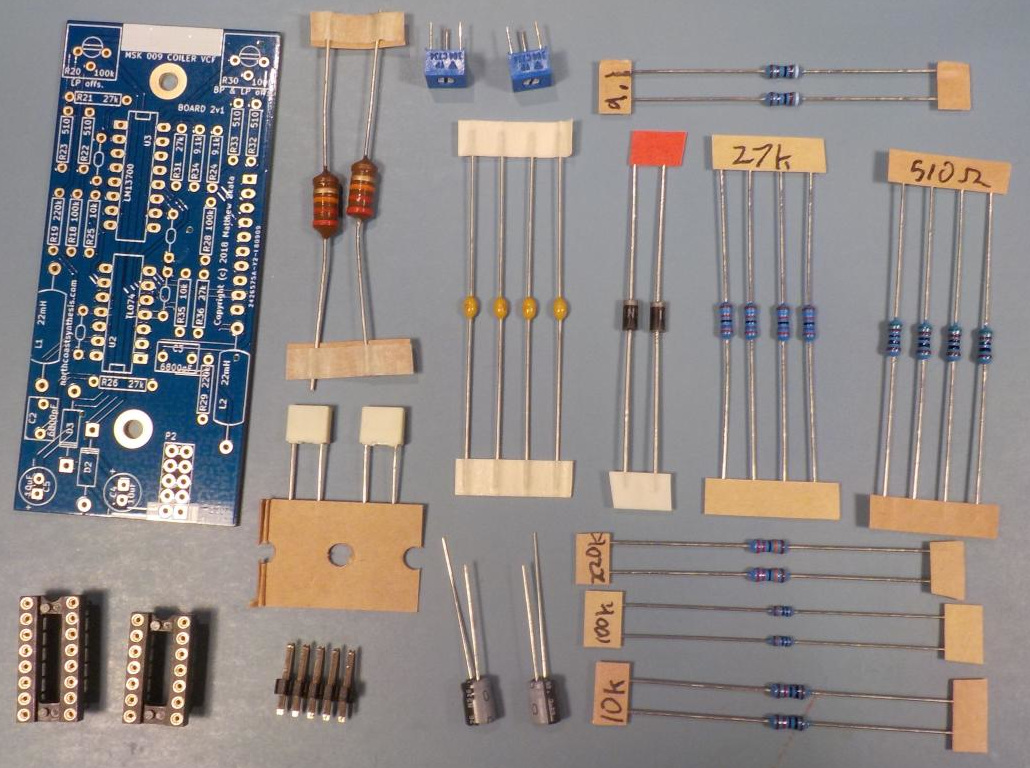
\includegraphics[width=\linewidth]{board2-parts.jpg}

There are two trimmers to be installed on this board.  Before
installing them, use an ohmmeter to adjust each one to 50\% of its range. 
Measure the resistance along the track, then measure the resistance from the
wiper to one end and adjust to make the wiper half the total track
resistance.  This need not be exact, but having them start near their
midpoints will help with adjustment later,
by reducing issues with interaction among the different settings.  With both
trimmers pre-set to 50\%, the module should basically work even if it is not
at its best, whereas if they are installed at extreme values instead, then
you may have trouble getting it up and running enough to adjust it more
accurately.

\begin{table*}
{\centering
\fbox{This table is not a substitute for the text instructions.}
\vspace{\baselineskip}

\begin{tabular}{rp{1.3in}cp{3in}}
  \textbf{Qty} & \textbf{Ref} & \textbf{Value/Part No.} & \\ \hline
\input{bomdata-2.tex}
\end{tabular}\par}
\caption{Bill of Materials for assembling Board~2.  Also needed is the PCB
itself.}\label{tab:b2bom}
\end{table*}

\section{Decoupling capacitors}

The four axial ceramic 0.1$\mu$F decoupling capacitors, C8 to C11, are shown
on the board by a special symbol without their reference designators.

\nopagebreak
\noindent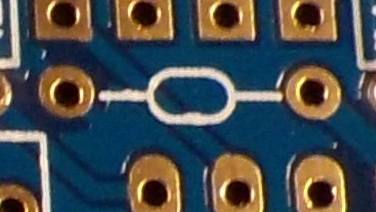
\includegraphics[width=\linewidth]{decoup-symbol.jpg}

Install these four capacitors where the symbol appears.  They are not
polarized and may be installed in either orientation.  These capacitors act
as filters for the power supplies to the op amp and OTA chips.  An MSK~009
kit should include six of these capacitors, and only four are used on this
board; save the remaining two for use on Board~1.

\nopagebreak
\noindent\includegraphics[width=\linewidth]{{cap-0.1u2}.jpg}

\section{Fixed resistors}

Resistors are never polarized.  I like to install mine in a consistent
direction for cosmetic reasons, but this is electrically unnecessary.  In
this module, the fixed resistors are metal film 1\%\ type.  They usually
have blue bodies and four colour bands designating the value, plus a fifth
band for the tolerance.  The tolerance band is brown for 1\%, but note that
we may occasionally ship better-tolerance resistors in the kits than the
specifications require, if we are able to source them at a good price. 
Accordingly, I mention only the four value band colours for this type of
resistor; if you are using resistors with other codes, you are responsible
for knowing them.  Note that colour codes on metal film 1\% resistors are
often ambiguous (reading from one end or the other end may give two
different values, both plausible) and some of the colours are hard to
distinguish anyway.  If in doubt, always measure with an ohmmeter before
soldering the resistor in place.

Install the four 510$\Omega$ (green-brown-black-black) resistors R22, R23,
R32, and R33.  These resistors, with the 100k$\Omega$ ones added later, set
the signal levels at the inputs of the OTA chips.

\nopagebreak
\noindent\includegraphics[width=\linewidth]{{res-510}.jpg}

\pagebreak
Install the two 9.1k$\Omega$ (white-brown-black-brown) resistors R24 and
R34.  These limit the maximum control current for the OTAs.

\nopagebreak
\noindent\includegraphics[width=\linewidth]{{res-9.1k}.jpg}

Install the two 10k$\Omega$ (brown-black-black-red) resistors R25 and R35. 
These are feedback resistors for the current-to-voltage converters in the
filter core.

\nopagebreak
\noindent\includegraphics[width=\linewidth]{{res-10k}.jpg}

\pagebreak
Install the four 27k$\Omega$ (red-violet-black-red) resistors R21, R26, R31, and R36. 
These are feedback resistors for the integrators (R26 and R36), and set the
current for the linearizing diodes in the LM13700 chips (R1 and R31).

\nopagebreak
\noindent\includegraphics[width=\linewidth]{{res-27k}.jpg}

Install the two 100k$\Omega$ (brown-black-black-orange) resistors R18 and
R28.  These resistors participate in setting the input levels for the OTA
chips.  A full kit contains seven resistors of this value; five should
remain for use on Board~1.

\nopagebreak
\noindent\includegraphics[width=\linewidth]{{res-100k2}.jpg}

Install the two 220k$\Omega$ (red-red-black-orange) resistors R19 and
R29.  These resistors set the adjustment ranges for the DC offset trimmers.
A full kit contains four
resistors of this value; save two for use on Board~1.

\nopagebreak
\noindent\includegraphics[width=\linewidth]{{res-220k2}.jpg}

\section{Semiconductors}

Install the two 1N5818 or SBA130 Schottky rectifier diodes D2 and D3.  These
are for reverse-voltage protection; they cut off power to the module when
the power plug is backwards.  They are polarized and it is important to
install them in the right direction.  Each diode is packaged inside a black
or dark grey plastic slug with a white or light grey stripe at one end; that
end is the \emph{cathode}.  The silkscreen markings on the board have a
corresponding stripe and the diodes should be installed with their stripes
matching the markings on the board.  The solder pads for the cathodes are
also square instead of round.  Installing these backwards means they will
have the opposite of the intended protective effect.

\nopagebreak
\noindent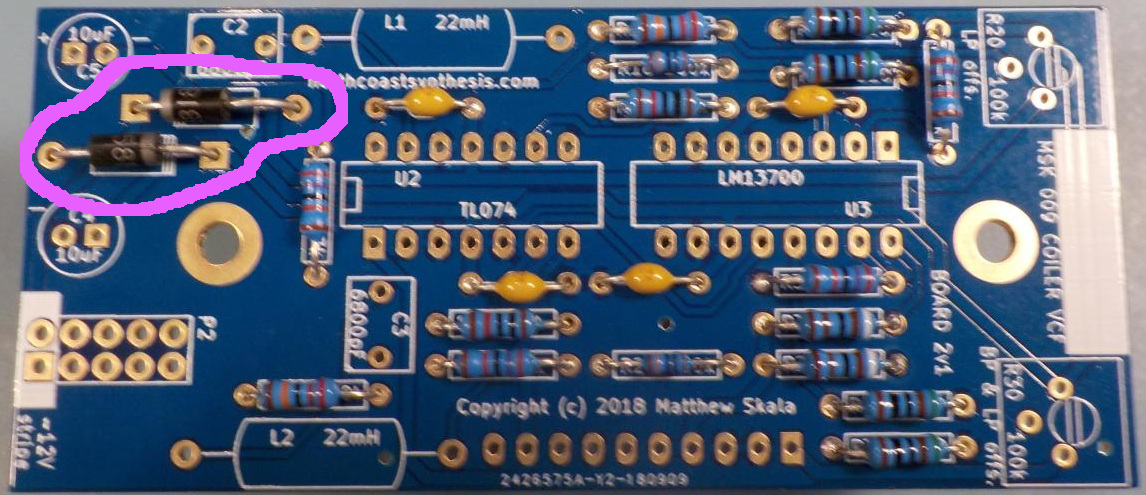
\includegraphics[width=\linewidth]{schottky.jpg}

Install the 14-pin DIP socket for the operational amplifier chip U2.  This
chip does most of the amplification in the filter core.  DIP sockets
themselves do not care which direction you install them, but it is
critically important that the chips installed in the sockets should be
installed in the right direction.  To help with that, the sockets will
probably be marked with notches at one end (indicating the end where Pin~1
and Pin~14 are located) and you should install the sockets so that the
notched ends match the notches shown on the PCB silkscreen.  The solder pad
for Pin~1 is also distinguished by being rectangular instead of rounded.

Installing DIP sockets without having them tilted at a funny angle can be
tricky.  I recommend inserting the socket in the board, taping it in place
on the component side with vinyl electrical tape or sticking it there with a
small blob of putty at each end, then soldering one pin on
one corner and checking that the socket is snug against the board before
soldering the other pins.  That way, if you accidentally solder the first
pin with the socket tilted, it will be easier to correct (only one pin to
desolder instead of all of them).

\nopagebreak
\noindent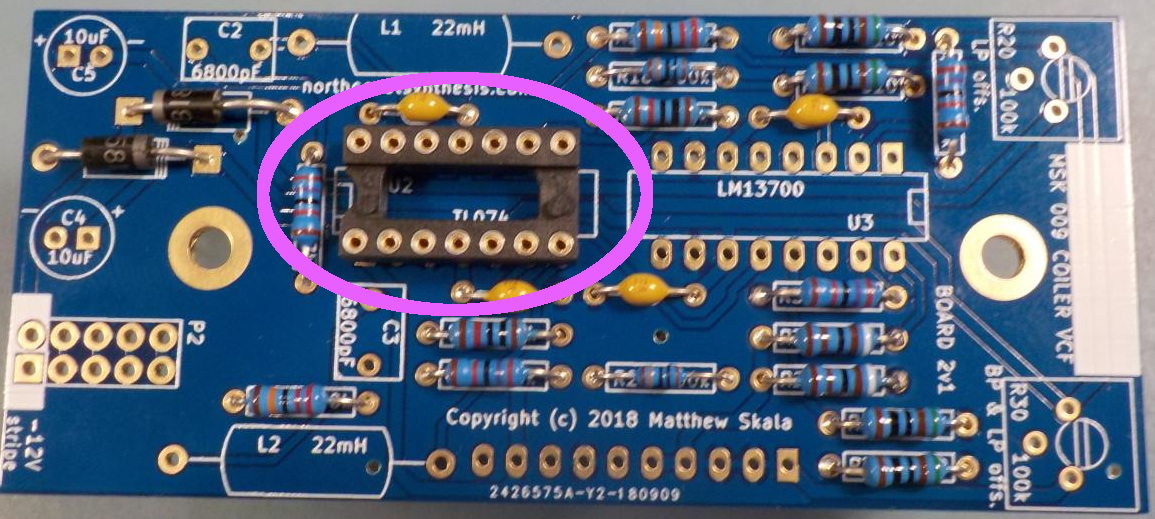
\includegraphics[width=\linewidth]{dip14-2.jpg}

If you somehow manage to solder an entire socket in backwards, don't try to
desolder it to turn it around.  Just leave it as it is and remember that
when you insert the chip, you must insert it so the chip matches the
markings on the \emph{board}, not the turned-around socket.

Install the 16-pin DIP socket for the OTA (operational transconductance
amplifier) chip U3.  This chip contains two current-controlled amplifiers,
which, by means of a frequency-dependent control current, tune the filter
core to the desired frequency.  See the general instructions regarding DIP
sockets above.

\nopagebreak
\noindent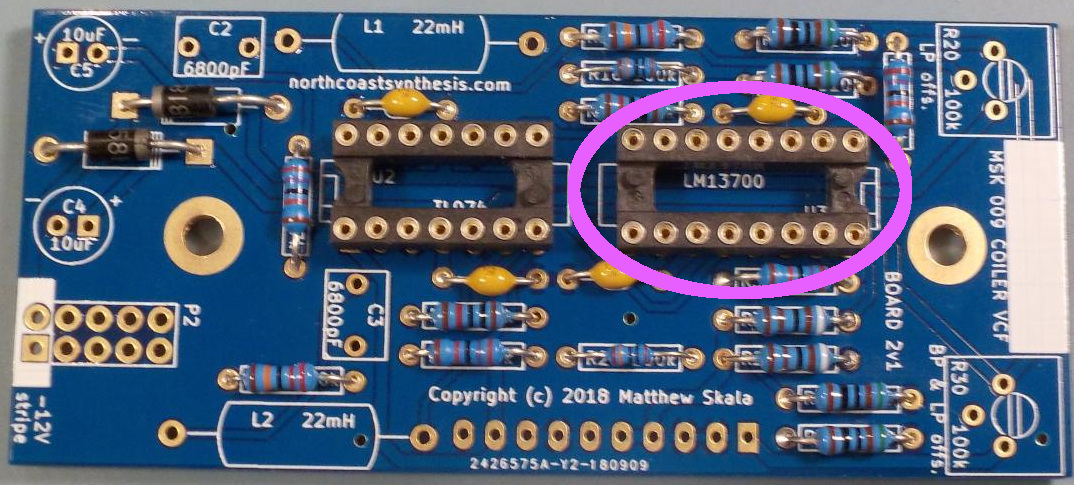
\includegraphics[width=\linewidth]{dip16.jpg}

\section{Electrolytic and film capacitors}

Install the two 6800pF film capacitors C2 and C3.  These are timing
components used in the integrators at low frequencies to complement the
inductors used at medium to high frequencies.  They are unpolarized
components and may be installed in either orientation.

The markings on film capacitors may vary depending on the manufacturer and
model.  These ones might be marked ``682'' (for 68 followed by two 0s number
of picofarads), ``6n8'' (for 6.8nF), or even ``0.0068'' (value in $\mu$F). 
However, these are the only film capacitors in the module, so confusion is
unlikely.

\nopagebreak
\noindent\includegraphics[width=\linewidth]{{cap-6800p}.jpg}

\pagebreak

Install the two 10$\mu$F electrolytic capacitors C4 and C5, which
filter the power supply for the module as a whole. 
These are polarized components and they may explode if installed backwards. 
Each one will be marked on its casing with a stripe and minus signs to
indicate the negative lead; the positive lead will probably also be longer. 
These clues should be matched with the markings on the PCB: plus and minus
symbols in the silkscreen and a square solder pad for the positive (long)
lead.

\nopagebreak
\noindent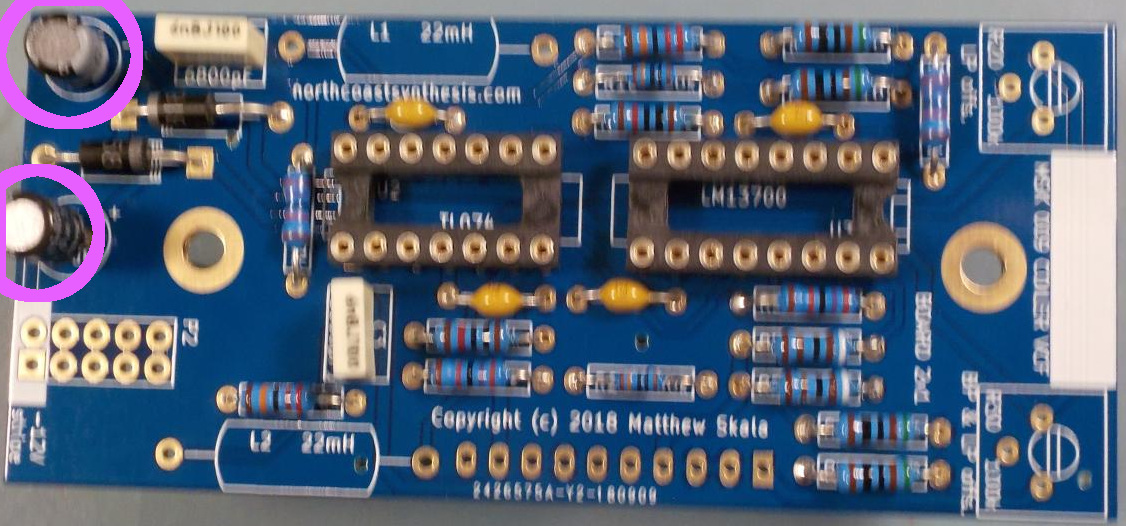
\includegraphics[width=\linewidth]{cap-10u.jpg}

\section{Trimmer potentiometers}

If you have not already set the trimmers to 50\%\ of their full scale value
as described under ``Preliminaries'' above, then do it now.

Trimmers usually are not washable, so if you plan to clean your boards by
full immersion in water or other solvent,
your last chance is now; future cleaning will have to
be done with a brush and some care to avoid letting liquid seep into the
trimmers.  Even now you should take some care with the DIP sockets, because
solvent can carry flux residue into them and form a varnish-like layer if
not carefully rinsed away.

Trimmers are not exactly polarized, but the three legs of each trimmer serve
different functions and need to be connected to the right holes.  The
physical arrangement of the legs and corresponding holes should make it
impossible to install the trimmers wrong way round.

Install the two 100k$\Omega$ trimmers R20 and R30.  These trimmers
are for compensating DC offsets in the filter core.

\nopagebreak
\noindent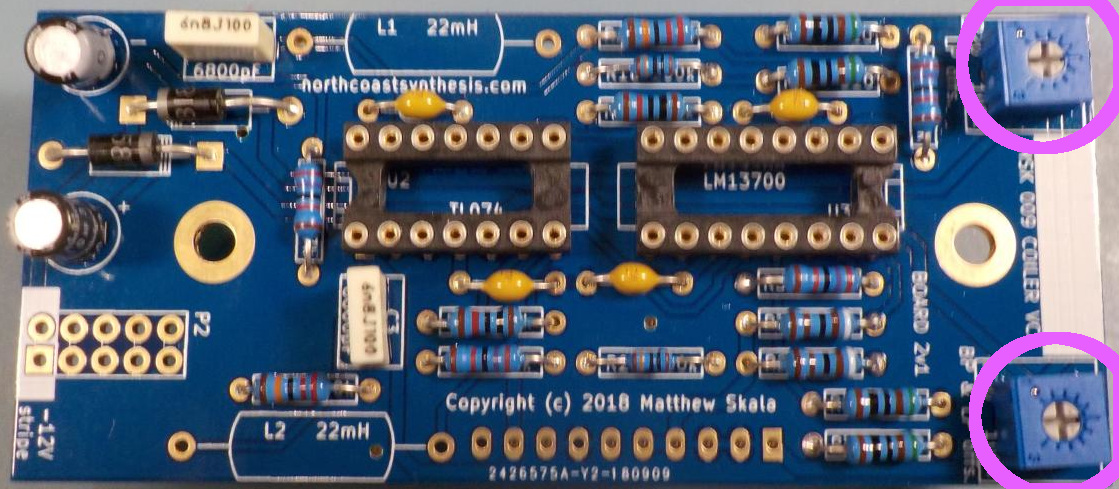
\includegraphics[width=\linewidth]{pot-100k2.jpg}

\pagebreak

\section{Inductors}

The two 22mH ferrite-bobbin inductors, that is, \emph{coils}, L1 and L2 give
this module its name.  Install them now.  They are the main timing
components in the filter core, serving at medium to high frequencies. 
Single inductors like these have no polarity and may be installed in either
direction; the situation is more complicated with transformers made of two
or more interacting inductors.

The inductors are delicate, especially in the area where the leads attach to
the bodies, because the windings that connect to the leads are made of very
fine wire.  The ferrite core material is also somewhat brittile.  It is
important not to bend the leads too close to the bodies.  There is some
extra space for the inductors on the circuit board to allow for a gentle
bend radius.

\nopagebreak
\noindent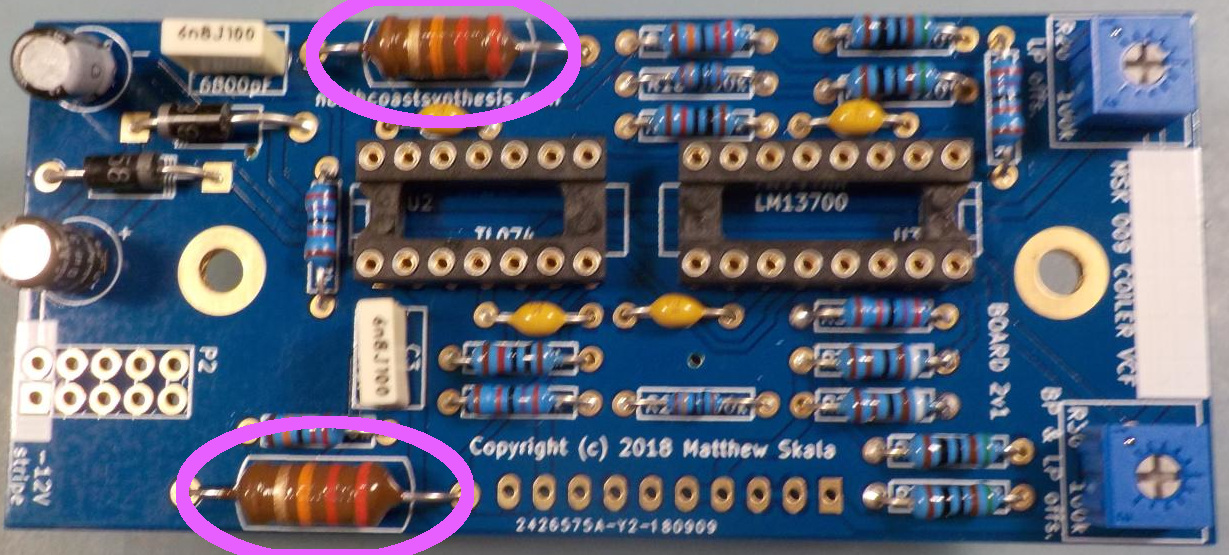
\includegraphics[width=\linewidth]{coils.jpg}

\section{Eurorack power connector}

Install the 2$\times$5-pin Eurorack power connector J2.  This connector is
not polarized in itself, although the connection it makes is polarized.  As
with the DIP sockets, you should be careful to get it installed snugly
against the board, not tilted at an angle.  Use tape or putty to
hold it in place, solder one pin, then check that it is straight before you
solder the other pins.

The six pins in the centre of the connector, that is all except the four
corner pins, are for grounding and they are all connected together on the
board.  Thus, if you accidentally form solder bridges among these six pins
while installing the connector, don't waste effort trying to remove them;
they will have no electrical effect.

\nopagebreak
\noindent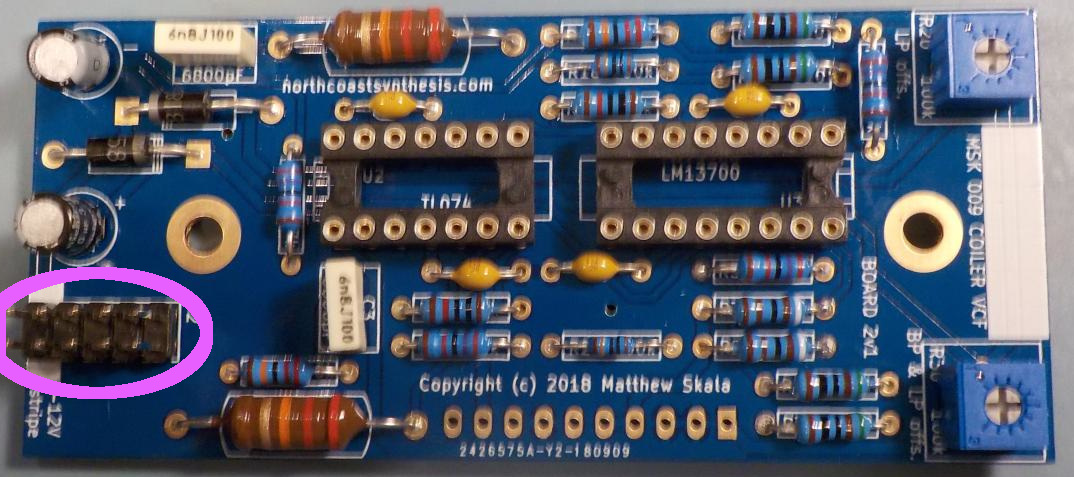
\includegraphics[width=\linewidth]{power.jpg}

In between completed boards is a good time to take a break.

